% 设定文章类型,正文字号为小四,若为五号将-4改为5即可
\documentclass[zihao=-4,UTF8]{report}		

% 导入基本宏包
\usepackage[UTF8]{ctex}     % 设置文档为中文语言
% \usepackage{hyperref} (此宏包与标题中的数学环境冲突)  % 宏包:自动生成超链接
\usepackage{amsmath}    % 宏包:数学公式
\usepackage{amssymb}    % 宏包:提供更多数学符号

% 文章页面margin设置
\usepackage[a4paper]{geometry}
\geometry{top=1in}
\geometry{bottom=1in}
\geometry{left=0.75in}
\geometry{right=0.75in}   % 设置上下左右页边距
\geometry{marginparwidth=1.75cm}    % 设置边注距离(注释、标记等)

%宏包:有色文本框及其设置
\usepackage[dvipsnames,svgnames]{xcolor}    %设置插入的文本框颜色
\usepackage[strict]{changepage}     % 提供一个 adjustwidth 环境
\usepackage{framed}     % 实现方框效果
\definecolor{formalshade}{rgb}{0.95,0.95,0.96} % 文本框颜色。修改此行中的 rgb 数值即可改变方框纹颜色,具体颜色的rgb数值可以在网站https://colordrop.io/中获得。(截止目前的尝试还没有成功过,感觉单位不一样)(找到喜欢的颜色,点击下方的小眼睛,找到rgb值,复制修改即可)
\newenvironment{formal}{%
\def\FrameCommand{%
\hspace{1pt}%
{\color{gray}\vrule width 2pt}%
{\color{formalshade}\vrule width 4pt}%
\colorbox{formalshade}%
}%
\MakeFramed{\advance\hsize-\width\FrameRestore}%
\noindent\hspace{-4.55pt}% disable indenting first paragraph
\begin{adjustwidth}{}{7pt}%
\vspace{2pt}\vspace{2pt}%
}
{%
\vspace{2pt}\end{adjustwidth}\endMakeFramed%
}

% chapter标题自定义设置
\usepackage{titlesec}   
\titleformat{\chapter}[hang]{\normalfont\huge\bfseries\centering}{第\,\thechapter\,章}{20pt}{\Huge}
\titlespacing*{\chapter}{0pt}{-20pt}{20pt} % 控制上方空白的大小

% table设置
\usepackage{float}
\usepackage{booktabs}
\usepackage{caption}

% 页眉页脚设置
\usepackage{fancyhdr}   %宏包:页眉页脚设置
\pagestyle{fancy}
\fancyhf{}
\cfoot{\thepage}
\renewcommand\headrulewidth{1pt}
\renewcommand\footrulewidth{0pt}
\chead{Linear Algebra Ⅰ Notes}    

%宏包:图片插入设置
\usepackage{graphicx}   
\usepackage{float}      
\usepackage{amssymb}    
\usepackage{caption}\captionsetup[figure]{name=图}  

% 文章默认字体设置
\usepackage{fontspec}   % 宏包:字体设置
\setmainfont{SimSun}    % 设置中文字体为宋体字体
\setmainfont{Times New Roman} % 设置英文字体为Times New Roman

% 参考文献引用设置
\bibliographystyle{unsrt}   % 设置参考文献引用格式为unsrt
\newcommand{\upcite}[1]{\textsuperscript{\cite{#1}}}     % 自定义上角标式引用

% 文章序言设置
\newcommand{\cnabstractname}{序言}
\newenvironment{cnabstract}{%
  \par\Large
  \noindent\mbox{}\hfill{\bfseries \cnabstractname}\hfill\mbox{}\par
  \vskip 2.5ex}{\par\vskip 2.5ex}

%文档作者信息设置
\title{线性代数Ⅰ笔记\\Linear Algebra Ⅰ Notes}
\author{丁毅\\ \footnotesize 中国科学院大学,北京 100049\\ Yi Ding \\ \footnotesize University of Chinese Academy of Sciences, Beijing 100049, China}
\date{\footnotesize 2023.10 - 2024.1}

% 开始编辑文章
\begin{document}
\maketitle
\newpage

\addcontentsline{toc}{chapter}{序言} % 手动添加为目录
\thispagestyle{fancy}   % 显示页码、页眉等
\begin{cnabstract}
\normalsize 本书为笔者本科时的代数笔记,包含线性代数和抽象代数中的常见内容,以及少部分拓展内容。本书用黑色表示笔记内容的主干框架,用灰色以及有色方框等表示对主干内容的补充、对晦涩概念的理解、定理的具体证明过程等,采用红色对重点知识进行强调,同时适当配有插图。这样的颜色和结构安排既突出了知识的主要框架,也保持了笔记的深度和广度,并且不会因为颜色过多而导致难以锁定文本内容,乃是尝试了多种安排后挑选出的最佳方案。如果读者有更佳的颜色和排版方案,可以将建议发送到笔者邮箱,在此感谢。\par
由于个人精力及知识水平有限,书中难免有不妥、错误之处,望不吝指正,在此感谢。
\end{cnabstract}
\pagenumbering{Roman} % 页码为大写罗马数字

\tableofcontents        % 目录页   

\newpage
\pagenumbering{arabic} 
\chapter{代数的起源}
\thispagestyle{fancy} 
\section{从代数起源到低阶行列式}

\textbf{一般方程根式解:}$n$次一般方程$(n\geq5)$没有根式解:
$a_{n}x^{n}+a_{n-1}x^{n-1}+...+a_{0}=0$\par

\textbf{对角矩阵}:$n$阶对角矩阵(diagnal matrix):
\begin{equation*}
    D=\begin{bmatrix}  a_{11}& 0 & ... & 0\\  0&  a_{22}&  \ddots&\vdots \\  \vdots & \ddots & \ddots 
 &\vdots  \\  0& ... & ... & a_{nn}\end{bmatrix}
\end{equation*}


当$a_{11}=a_{22}=...=a_{nn}=a$时,$\mathit{D}$称为纯量矩阵,记为$diag_{n}(a)$,其中$diag$指代英文中的diagnal (adj.对角的)。矩阵$diag_{n}(1)$称为$n$阶单位矩阵(identity matrix of order n),记作$I_{n}$或$I$。\par

\textbf{低阶行列式:}一阶、二阶、三阶行列式(略)

\section{集合(set)与映射(map)}
\subsection{集合的相关概念}

\textbf{差集:}
$X$\textbackslash $Y$或$X-Y$,表示集合$\left \{x\mid x\in X,x\notin Y \right \} $。

\textbf{笛卡尔积:}
\(X \times Y=\left \{(x,y)\mid x\in X,x\in Y \right \} \),$n$阶笛卡尔积:$X^n=X\times X\times X...X$($n$个$X$相乘)

\textbf{集合的势(基数):}
设$X,Y$为两集合,如果存在双射$f:X\to Y$,则称$X$与$Y$等势(或有相同的基数),记为$cardX=cardY$,或$X\sim Y$。其中$card$代指英文中的cardinal(n.基数)。容易证明,基数满足如下运算,设$X$为$n$元集合,$Y$为$m$元集合,则有:
$\left |X \right | = cardX=n\text{,}\left |  Y \right |= cardY =m\text{,}\left | X\times Y \right | =card(X\times Y)=nm$,
$\left | X\cup Y \right |+\left | X \cap  Y \right |=n+m$.

\textbf{容斥原理:}
$\left | S\cup T \right | +\left | S\cap T \right | =\left | S \right | +\left | T \right |$ 

\textbf{映射的原像与像:}
“原像”即为映射$f$的定义域,也就是$X$,“像”即为映射$f$的值域,并且值域$Im(f)\subseteq  Y$,当且仅当$f$为满射时取等。$Im(f)$表示映射$f$的值域,也可以用$f(X)$表示$f$的值域。

\textbf{映射的逆:}
\begin{align*}
    &f\text{有逆}\iff f\text{为双射}\\
    &f\text{有左逆}\iff f\text{为单射}\\
    &f\text{有右逆}\iff f\text{为满射}\\
    &\text{若映射}f\text{有逆,则逆唯一}
\end{align*}

\textbf{集合的幂集:}
集合$X$的所有子集构成的集合称为$X$的幂集,记为$\mathcal{P}(X)$.

\section{二元关系与商映射}
\subsection{二元关系}
\textbf{二元关系定义:}给定两个集合$X,Y$,且$\omega \subset X\times Y$,则称$\omega$为$X,Y$之间的一个二元关系。若$(x,y)\in \omega $,则称$x,y$有二元关系$\omega$,记为$x\omega y$.\par
\textcolor{gray}{对二元关系定义的理解:给定集合$X=\left \{ \text{喜羊羊,沸羊羊,美羊羊,灰太狼,红太狼} \right \} $,定义$\heartsuit =\left \{ \text{(沸羊羊,美羊羊),(美羊羊,喜羊羊),(灰太狼,红太狼),(红太狼,灰太狼)}\right \} $,显然$\heartsuit$是$X,Y$之间的一个二元关系,且对沸羊羊,美羊羊$\in X$,有沸羊羊$\heartsuit $美羊羊,但是反之则不成立,也即美羊羊$\heartsuit $沸羊羊不成立。}

\subsection{等价关系}
\textbf{等价关系定义:}等价关系是一种(一类)特殊的二元关系。满足下面三条性质的二元关系称为等价关系.
\begin{align*}
    &\text{反身性(自反性):}x\sim x\\
    &\text{对称性:}x\sim y \Longrightarrow y\sim x\\
    &\text{传递性:}x\sim y\text{,}y\sim z \Longrightarrow x\sim z
\end{align*}

\textbf{等价类:}
设$\sim $是$X$上的一个等价关系,对元素$x \in X$,定义$X$关于$\sim $的、含有元素$x$的等价类为$\bar{x} =\left \{x\in X\mid x \sim x' \right \}$

\textbf{商集:}
$X$关于等价关系$\sim$的全体等价类构成的集合称为$X$关于$\sim$的商集,记为$X/\sim $

\textbf{划分:}
通过某种依据,将集合$X$分为数份并构成新集合,这个新集合叫作$X$的一种划分。且有定理:$X$上的等价关系与它的划分一一对应

\subsection{偏序关系}
\textbf{偏序关系定义:}
偏序关系是一种特殊的二元关系$\omega$。满足下面三条性质的二元关系称为偏序关系.
\begin{align*}
    &\text{反身性(自反性):}x\sim x\\
    &\text{反对称性:}x\sim y,\;y\sim x \Longrightarrow y=x\\
    &\text{传递性:}x\sim y,\;y\sim z \Longrightarrow x\sim z
\end{align*}

\textbf{可比:}
$x,y\in A,x$与$y$可比$\Longleftrightarrow x\preceq y $或 $y\preceq x$

\textbf{全序(集):}
全序是一种特殊的偏序关系。若集合$X$上的一个偏序关系$\preceq_{0}$满足:$\forall x,y\in A, $都有$x,y$可比,也即$\forall x,y\in A, $有$x\preceq_{0}y$ 或$y\preceq_{0}x$,则称偏序关系$\preceq_{0}$为全序,同时称集合$X$为全序集。

\textbf{覆盖:}
$x,y\in A ,x \preceq y $, 若不$\exists z \in A $使得$x\preceq z\preceq y$, 则称$y$覆盖$x$.\par
\textcolor{gray}{例如$A=\left \{ 1,2,4,9 \right \} $上的整除关系,9覆盖1,4覆盖2,4不覆盖1}

\textbf{偏序集:}
由集合$A$和$A$上的一个偏序关系构成的``数对'',称为偏序集,记作$(A,\preceq)$\par
\textcolor{gray}{如$(\mathbb{N}, \le )$和$(\mathcal{P}(A) , \subseteq)$,其中$\mathcal{P}(A)$表示$A$的全体子集构成的集合。}

\textbf{偏序图(哈赛图):}\par
哈赛图是一种简化的偏序关系图(一般由下向上看),以$(\left \{ 1,2,3,4,5,6,7 \right \},\text{整除} )$的哈赛图为例:
\begin{figure}[H]
    \centering
    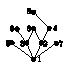
\includegraphics[scale=4]{../pic/位图.pdf}
    \caption{哈赛图示例}
\end{figure}

\section{置换}

\subsection{置换的基本概念}

\textbf{置换的定义:}
置换是由$X\longrightarrow X$的一个双射,其中$X$为$n$元有限非空集合。\par
\textcolor{gray}{可以思考一下“置换”和“排列”之间的联系}

\textbf{对称群的定义:}
$n$元有限非空集合$X$的全体置换构成集合$S_{n}$,称$S_{n}$为集合$X$上的对称群。且易证:
\begin{equation*}
    \left | S_{n} \right | =card(S_{n})=n!
\end{equation*}

\textbf{置换的乘法(置换的复合):}
关键思路:``谁变成谁"。满足结合律,不一定满足交换律。
\begin{align*}
    \text{设}\sigma &=
    \begin{pmatrix}
    1&  2&  3& 4\\
    2&  3&  4&1
    \end{pmatrix} ,
\nu =
    \begin{pmatrix}
    1&  2&  3& 4\\
    4&  3&  2&1
    \end{pmatrix}\text{,则:}\\
    \sigma \nu &= 
        \begin{pmatrix}
        1&  2&  3& 4\\
        2&  3&  4&1
        \end{pmatrix}
        \begin{pmatrix}
            1&  2&  3& 4\\
            4&  3&  2&1
        \end{pmatrix}=
        \begin{pmatrix}
            1&  2&  3& 4\\
            4&  2&  1& 3
        \end{pmatrix}\\
     \nu \sigma &= 
        \begin{pmatrix}
            1&  2&  3& 4\\
            4&  3&  2&1
        \end{pmatrix}
        \begin{pmatrix}
            1&  2&  3& 4\\
            2&  3&  4&1
        \end{pmatrix}=
        \begin{pmatrix}
            1&  2&  3& 4\\
            1&  3&  4& 2
        \end{pmatrix}
\end{align*}\par
\textcolor{gray}{注意:置换乘法从右向左计算(置换是一个双射,想想映射的复合)}


\textbf{循环:}
设置换$\sigma$是一个循环,如果$\sigma$``移动了''$X$中的$r$个元素,则称$\sigma $为$r$循环(常写作$r-cycle$),记为$\sigma=(i_{1},i_{2},...,i_{r})$,且可以用循环图表示,举两个例子:
\begin{align*}
    \sigma &= 
    \begin{pmatrix}
        1&  2&  3& 4\\
        2&  3&  1& 4
    \end{pmatrix}=
    \left ( 1\;2\;3\right ) \text{为$3-cycle$,如图1.2}\\
    \nu &= 
    \begin{pmatrix}
        1&  2&  3& 4& 5\\
        5&  1&  4& 2& 3
    \end{pmatrix}=
    \left ( 1\;5\;3\;4\;2\right )\text{为$5-cycle$,如图1.3}
\end{align*}
\begin{minipage}[b]{0.45\columnwidth}
    \begin{figure}[H]
        \centering
        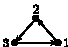
\includegraphics[scale=3]{../pic/循环图1.pdf}
        \vspace{10pt}
        \caption{$\sigma=\left ( 1\;2\;3\right )$循环图}
    \end{figure}
\end{minipage}
\begin{minipage}[b]{0.48\columnwidth}
    \begin{figure}[H]
        \centering
        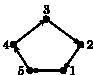
\includegraphics[scale=3]{../pic/循环图2.pdf}
        \caption{$\nu=\left ( 1\;5\;3\;4\;2\right )$循环图}
      \end{figure}
\end{minipage}



特别地,不移动(即固定)所有元素的循环为1循环,也即恒等置换(恒等变换)。一个$2-cycle$仅交换$X$中的一对元素,故称为对换。

\textbf{循环的乘法(复合):}
循环的乘法可按置换乘法来做:
\begin{align*}
\begin{pmatrix}
    1&2
\end{pmatrix}
\begin{pmatrix}
    1&3&4&2&5
\end{pmatrix}
&=\begin{pmatrix}
    1&2&3&4&5\\
    2&1&3&4&5
\end{pmatrix}
\begin{pmatrix}
    1&2&3&4&5\\
    3&5&4&2&1
\end{pmatrix}
=
\begin{pmatrix}
    1&2&3&4&5\\
    3&5&4&1&2
\end{pmatrix}\\
&=\begin{pmatrix}
    1&3&4
\end{pmatrix}
\begin{pmatrix}
    2&5
\end{pmatrix}
\end{align*}
也可以按照循环的意义来做:从右向左依次复合,谁变成谁、再变成谁。\par
\textcolor{gray}{从右向左算,得到哪个数字就继续看这个数字的变化,如得到“(14”下一步便看4变成了谁,直至形成闭环,打上右括号。然后为避免遗漏,从小到大考虑暂未变换的数。}

\textbf{置换相交/不相交:}
两个置换$\sigma_{1},\sigma_{2}$称为不相交的如果:$\forall i \in \left \{ 1,2,...,n \right \},i $至多被$\sigma_{1},\sigma_{2}$中的一个置换移动。反之则称$\sigma_{1},\sigma_{2}$相交。另外,由于置换可以通过置换基本定理写为循环乘积的形式,那么不相交可等价的定义为:两个置换的循环表示中不存在相同元素。

\textbf{置换的奇偶性:}
若一个置换$\sigma$以写成奇数(偶数)个对换的乘积,则称置换$\sigma$为奇置换,并定义符号:
\begin{equation*}
\varepsilon_{\sigma}=
\left\{\begin{matrix}
    -1&, \sigma \text{为奇置换}\\
    1&, \sigma \text{为偶置换}
\end{matrix}\right.
\end{equation*}
由置换基本定理、循环的对换分解,有结论:
\begin{align*}
    \varepsilon_{\sigma}=(-1)^{\sum_{i=1}^{m} (r_{i}-1)},\varepsilon_{\sigma \nu}=\varepsilon_{\sigma}\varepsilon_{\nu} 
\end{align*}


\textbf{置换的逆:略}

\textbf{置换的阶:}
对于一个置换$\sigma \in S_{n}$,若$\sigma^{p}=e$,则称$\sigma$为一个$p$阶置换。且有定理:
\begin{equation*}
    \forall \; r-cycle \; \sigma \in S_{n},\; \text{有}\sigma ^{r}=e
\end{equation*}\par
也即$r-cycle$是一个$r$阶循环。再由置换基本定理,可推得:
\begin{equation*}
    \forall \; \sigma=
    \begin{pmatrix}
        i_{1}&i_{2}&...&i_{r_{1}}
    \end{pmatrix}
    ...
    \begin{pmatrix}
        j_{1}&j_{2}&...&j_{r_{s}}
    \end{pmatrix}
    ,\; \sigma \text{的阶数为}\; p=l.c.m(r_{1},r_{2},...,r_{n})
\end{equation*}\par
\textcolor{gray}{补充:\,$S_{n}$中元素的最高阶为$m=l.c.m(1,2,3,...,n)$,\,经查阅资料,\,$l.c.m(1,2,3,...,n)=f(n)$为$Landau's function$,\,渐近于$e$}

\textbf{置换作用于函数:}\par
设$f(x_{1},x_{2},...,x_{n})$为$n$元函数,定义:$\sigma \circ f(x_{1},x_{2},...,x_{n})=f(x_{\sigma(1)},x_{\sigma(2)},...,x_{\sigma(n)})$

\textbf{对称/斜对称函数:}
对称函数:一个定义在$X^{n}$上的函数称为对称的如果:
\begin{equation*}
    \forall \; x_{i},x_{j}\in I, f(x_{1},x_{2},...,x_{i},...,x_{j},...,x_{n})=f(x_{1},x_{2},...,x_{j},...,x_{i},...,x_{n})
\end{equation*}\par
上述定义可等价地写为:
\begin{equation*}
    \forall \; \sigma \in S_{n},\sigma \circ f=f
\end{equation*} \par
斜对称函数:一个定义在$X^{n}$上的函数称为斜对称的如果:
\begin{equation*}
    \forall \; x_{i},x_{j}\in I, f(x_{1},x_{2},...,x_{i},...,x_{j},...,x_{n})=-f(x_{1},x_{2},...,x_{j},...,x_{i},...,x_{n})
\end{equation*}\par

\textcolor{gray}{
常见的对称函数如:
\begin{align*}
    f(x_{1},x_{2},...,x_{n})=\sum_{i=1}^{n}x_{i}^{2},\quad g(x_{1},x_{2},...,x_{n})=\sum_{1\le i\le j\le n}x_{i}x_{j}=\sum_{j=1}^{n}\sum_{i=1}^{j}x_{i}x_{j}
\end{align*}
}\par
\textcolor{gray}{
常见的斜对称函数如$n$元列向量行列式($n$元行向量行列式同理):
    \begin{equation*}
        det(\vec{x}_{1}\vec{x}_{2},...,\vec{x}_{n})=
        \begin{vmatrix}
        \vec{x}_{1}&  \vec{x}_{2}& ... &\vec{x}_{n}
        \end{vmatrix}=
        \begin{vmatrix}
            x_{11} & x_{12} & ... & x_{1n}\\
            \vdots &  \vdots & \ddots  & \vdots \\
            x_{n1} & x_{n2} & ... & x_{nn}
        \end{vmatrix},\;
    \vec{x}_{i}=
    \begin{bmatrix}
        x_{1i}\\
        \vdots\\
        x_{ni}
    \end{bmatrix}\text{为}n\text{维列向量}
    \end{equation*}
}


\subsection{与置换相关的定理/推论}

\textbf{置换基本定理:}
每一个非恒等置换都可分解为数个不相交的循环之积,且这样的分解唯一(不考虑顺序),也即:
\begin{equation*}
    \forall \; \sigma \in S_{n},\; \exists \; \text{唯一确定的循环}\;{\nu_{1},\nu_{2},...,\nu_{n}} \;\text{满足:}\sigma=\nu_{1}\nu_{2}...\nu_{n}
\end{equation*}

\textbf{循环的对换分解:}
对任意长度为$r$的循环$\nu$,$\nu$ 可以写为$(r-1)$个对换的乘积,也即:
\begin{equation*}
    \nu=\begin{pmatrix}
        i_{1}&i_{2}&...&i_{r}
    \end{pmatrix}
    =\begin{pmatrix}i_{1}&i_{r}\end{pmatrix}\begin{pmatrix}i_{1}&i_{r-1}\end{pmatrix}...\begin{pmatrix}i_{1}&i_{2}\end{pmatrix}
\end{equation*}\par
这里要注意是倒序:从$r$到$2$。并且由此可以推得任意置换的对换分解,略。

\textbf{奇偶置换个数相同:}
一个$n$元对称群$S_{n}$中,全体奇置换$\overline{S_{n}}$与全体偶置换$\underline{S_{n}} $的个数相同,即$card\;\overline{S_{n}}=card\;\underline{S_{n}}=\frac{n!}{2} $

\textbf{置换的共轭作用:}
$\forall\;\sigma,\;\nu \in S_{n},\;\text{设}\;\nu=(i_{1}\;i_{2}\;...\;i_{r_{1}})...(j_{1}\;j_{2}\;...\;j_{r_{s}})$,有:
\begin{equation*}
    \color{red}
    \sigma \nu \sigma^{-1}=
    \begin{pmatrix}
        \sigma(i_{1})&\sigma(i_{2})&...&\sigma(i_{r_{1}})
    \end{pmatrix}
    ...
    \begin{pmatrix}
        \sigma(j_{1})&\sigma(j_{2})&...&\sigma(j_{r_{s}})
    \end{pmatrix}
\end{equation*}
\vspace{-30pt}
\begin{formal}
    \textbf{证明:置换的共轭作用}\par
    先证$\nu$为循环的情况。设
    $\nu=
    \begin{pmatrix}
        i_{1}&i_{2}&...&i_{r}
    \end{pmatrix}$
    ,则知$i_{1},i_{2},...,i_{r}\in \left \{ 1,2,...,n \right \} $,设$k\in \left \{ 1,2,...,n \right \}$,下面分类:\par
    当$\sigma^{-1}(k)\in \left \{ 1,2,...,n \right \}\setminus \left \{ i_{1},i_{2},...,i_{r} \right \}$时,
$\nu$不移动$\sigma^{-1}(k)$,即:
    \begin{equation*}
        \nu \sigma^{-1}(k)=\nu (\sigma^{-1}(k))=\sigma^{-1}(k)\Longrightarrow \sigma \nu \sigma^{-1}(k)=\sigma(\nu \sigma^{-1}(k))=\sigma \sigma^{-1}(k)=e(k)
    \end{equation*}\par
    当$\sigma^{-1}(k)\in \left \{ i_{1},i_{2},...,i_{r} \right \}$时,设$\sigma^{-1}(k)=i_{s},\;s\in \left \{ 1,2,...,r \right \}$,则$k=\sigma(i_{s})$,有:
    \begin{align*}
        s \le &r-1\;\text{时:}\\
        &\nu(\sigma^{-1}(k))=\nu(i_{s})=i_{s+1} \Longrightarrow \sigma\nu\sigma^{-1}(\sigma(i_{s}))=\sigma \nu \sigma^{-1}(k)=\sigma(\nu(\sigma^{-1}(k)))=\sigma(i_{s+1})\\
        s = &r\;\text{时:}\\
        &\nu(\sigma^{-1}(k))=\nu(i_{r})=i_{1} \Longrightarrow \sigma\nu\sigma^{-1}(\sigma(i_{s}))=\sigma \nu \sigma^{-1}(k)=\sigma(\nu(\sigma^{-1}(k)))=\sigma(i_{1})\\
        \text{于是}&\sigma^{-1}(k)\in \left \{ i_{1},i_{2},...,i_{r} \right \}\text{时,令}g=\sigma\nu\sigma^{-1},\text{则有:}g(\sigma(i_{s}))=
    \left\{\begin{matrix}
       \sigma(i_{s+1})&,s \le r-1\\
       \sigma(i_{1})&,\;\;s\;=\;r\;\;
      \end{matrix}\right.
    \end{align*}\par
    \par
    综上,写为循环形式即得:
    \begin{equation*}
        \sigma \nu \sigma^{-1}=
        \begin{pmatrix}
            \sigma(i_{1})&\sigma(i_{2})&...&\sigma(i_{r})
        \end{pmatrix}
    \end{equation*}\par
    再由置换基本定理进行推广,命题得证。
\end{formal}

\section{整数的算术}

\subsection{与整数相关的定理/推论}

\textbf{算术基本定理:}
$\forall\;n\in \mathbb{N}_{+},\;n\ge 2,\;\exists \text{!}\;p_{1},p_{2},...,p_{r},k_{1},k_{2},...,k_{r},\text{其中}p_{i}\text{为素数}, k_{i}\in  \mathbb{N}_{+}$,使得:
\begin{equation*}
    n=p_{1}^{k_{1}}p_{2}^{k_{2}}...p_{r}^{k_{r}}
\end{equation*}


\textbf{欧几里得定理:}
素数有无穷多个。

\textbf{带余除法:}
$\forall a,b\in \mathbb{N},\;\exists \text{!}q,r\in  \mathbb{N}$使得$a=bq+r$,其中$0\le r < b$

\textbf{欧几里得算法(辗转相除法):}
$\forall\; a,b\in \mathbb{N}_{+},$令$r_{0}=a,r_{1}=b$并定义$r_{i}=q_{i+1}r_{i+1}+r_{i+2}$,其中$0\le r_{i+2}< r_{i+1}$,则存在最小的整数$n$使得$r_{n+2}=0$,且有$r_{n+1}=g.c.d(a,b)$



\textbf{定理:}
三个整数的最大公因数与最小公倍数满足如下结论:
\begin{align*}
    g.c.d(a,b,c)=g.c.d(a,g.c.d(b,c))&&l.c.m(a,b,c)=l.c.m(a,l.c.m(b,c))
\end{align*}

\textbf{互质定理:}
$\forall \;m,n\in \mathbb{Z},mn\ne 0,\exists\; s,t\in Z,$使得$g.c.d(m,n)=s\left | m \right |+t\left | n \right | $
。特别地,当$m,n$互质时,$g.c.d(m,n)=1$,于是得到互质定理:正整数$m,n$互质$\Longleftrightarrow \exists\; s,t\in Z,$使得$sm+tn=1 .$\par

{\color{gray}
补充:由欧几里得算法求互质定理中的整数$s,t$\par
以$g.c.d(54,20)$为例,作辗转相除如下:\par
\begin{minipage}[c]{0.35\columnwidth}
    \begin{table}[H]
        \color{gray}
        \centering
        \begin{tabular}{l} 
        \toprule
        $r_0=54$,$r_1=20$ \\ 
        \hline
        $r_0 = q_1r_1+r_2$ \\
        $\Longrightarrow q_1 = 2$,$r_2=14$  \\
        \hline
        $r_1 = q_2r_2+r_3$ \\
        $\Longrightarrow q_2 = 1$,$r_3=6$  \\
        \hline
        $r_2 = q_3r_3+r_4$ \\
        $\Longrightarrow q_3 = 2$,$r_4=2$  \\ 
        \hline
        $r_3 = q_4r_4+r_5$ \\
        $\Longrightarrow q_4 = 3$,$r_5=0$  \\ 
        \bottomrule\\
        $\Longrightarrow g.c.d(54,20)=r_4=2$
        \end{tabular}
    \end{table}
\end{minipage}
\begin{minipage}[c]{0.54\columnwidth}
    \begin{align*}
        g.c.d(54,20)&=r_4\\
        &=r_2-q_3r_3\\
        &=r_2-q_3(r_1-q_2r_2)\\
        &=-q_3r_1+(1+q_2q_3)r_2\\
        &=-q_3r_1+(1+q_2q_3)(r_0-q_1r_1)\\
        &=(1+q_2q_3)r_0+(-q_1-q_1q_2q_3-q_3)r_1\\
        \Longrightarrow &
        \begin{cases}
            s=1+q_2q_3=3\\
            t=-q_1-q_1q_2q_3-q_3=-8
        \end{cases}
    \end{align*}
\end{minipage}
} 

\section{第一章思考题}
\textbf{1.\;$\forall\;r-cycle\;\sigma\in S_{n},$是否有$\sigma^{r}=e$?}
\begin{formal}
    \textbf{解:1.\;$\forall\;r-cycle\;\sigma\in S_{n},$是否有$\sigma^{r}=e$?}\par 
    容易证明,$\forall\;r-cycle\;\sigma \in S_n$,有$\sigma^r=e$,因此$r-cycle$也是一个$r$阶置换。
\end{formal}


\chapter{矩阵(matrices)}
\thispagestyle{fancy} 
\section{向量空间}
\subsection{向量空间的基本概念}

\textbf{$n$维向量空间:}\par
我们将向量与其直角坐标等同,则$n$维向量空间$ \mathbb{R}^{n}=\left \{\vec{x}= (x_{1},...,x_{n})\;|\;x_{1},x_{2},...,x_{n}\in \mathbb{R} \right \} $是一个由向量组成的集合,且容易验证其对线性运算封闭,称为$n$维向量空间,更严谨的称法是“$n$维欧式几何空间”。\par
\textcolor{gray}{$n$维向量空间是线性空间(vector space)的一种,下面我们给出线性空间的定义。}\par
\textcolor{gray}{
设$F$是域,$V$是一集合。在$V$中定义运算加法:
\begin{equation*}
    \forall \;v,u\in V,\;\exists\,!\; \mu \in V \,\text{使}\;\mu = v+u 
\end{equation*}
\indent 且$(V,\;+)$构成$Abel$群(也即:$V$对加法封闭,满足加法结合律和交换律,具有加法单位元,任意元素对加法可逆)。在$F,V$之间定义数乘:
\begin{equation*}
    \forall \;a\in F,\;v \in V,\;\exists\,!\; u \in V \,\text{使}\;u = a\cdot v 
\end{equation*}
\indent 且构成数乘满足结合律、具有单位元,加法和数乘满足左右分配率。此时称集合$V$是域$F$上的线性空间,$F$中的元素称为纯量或数量,$V$中的元素称为向量。在本书中,如无特别说明,我们的“向量空间”都指的是“$n$维欧氏几何空间”。}\par
\textcolor{gray}{下面是一些常见的线性空间:}\par
\textcolor{gray}{实数域上的全体$m$行$n$列矩阵构成一个线性空间,称为实数矩阵空间,记为$M_{m\times n}(\mathbb{R}) $。}\par
\textcolor{gray}{实区间$\left[a,b\right]\subseteq \mathbb{R}$上的全体连续函数构成一个线性空间,称为连续函数空间,记为$C_{\left[a,b\right]}$。}

\textbf{子空间:}
若$n$维向量空间$ \mathbb{R}^{n}$的非空子集满足$V$满足:$\forall \;\vec{a},\vec{b}\in V,\alpha ,\beta \in \mathbb{R},\; (\alpha  \vec{a}+\beta\vec{b})\in V  $,则称$V$为$ \mathbb{R}^{n}$的子空间。\par
\textcolor{gray}{容易证明,$\forall\;n\ge2,\mathbb{R}^{n}$有无数个子空间。}

\textbf{向量组的线性张成$Span$:}
设有限集$A=\left \{ \vec{a}_{1},\vec{a}_{2},...,\vec{a}_{n} \right \}\subset \mathbb{R}^{n} $,定义$A$的线性张成:
\begin{equation*}
    Span\;A=\left \{  \alpha_{1}\vec{a}_{1}+\alpha_{2}\vec{a}_{2}+...+\alpha_{n}\vec{a}_{n}\;|\; \alpha_{1}, \alpha_{2},..., \alpha_{n} \in \mathbb{R} \right \} 
\end{equation*}
有的教材也记作$Span(A)$。\par
容易验证,$Span\;A$是$ \mathbb{R}^{n}$的一个子空间。且有推论:设$U,V$为$ \mathbb{R}^{n}$的两个子空间,则$U\cap V$和$U+V$也是$ \mathbb{R}^{n}$的一个子空间,但$U\cup V$不一定是子空间。\par
\textcolor{gray}{特别地,我们有:$\mathbb{R} = Span \left \{ \vec{e}_{1},\vec{e}_{2},...,\vec{e}_{n} \right \} $}

\textbf{线性方程组、$ \mathbb{R}^{n}$、行列式间的联系:}
定理:$m$行$n$列齐次线性方程组$A\vec{x}=\vec{0}$的解集$X=\left \{ \vec{x}\;|\;A\vec{x}=\vec{0} \right \} $构成$\mathbb{R}^{n}$的子空间。\par
定理:$m$行$n$列线性方程组$A\vec{x}=\vec{b}$有解$\Longleftrightarrow \vec{b}\in Span\;A$\par
定理:若$m=n$,且行列式$det(A)\ne 0$,则$\forall\;\vec{b}\in \mathbb{R}^n$,方程$A\vec{x}=\vec{b}$有唯一解

\textbf{线性相关:}
设向量组$A=\left \{ \vec{a}_1,\vec{a}_2,...,\vec{a}_n \right \} $,其中$\vec{a}_i\in \mathbb{R}^m$,若存在不全为零的常数$\alpha_1,\alpha_2,...,\alpha_n$使得$\alpha_1\vec{a}_1+\alpha_2\vec{a}_2+...+\alpha_1\vec{a}_n=\vec{0}$,则称向量组$A$线性相关。\par
\textcolor{gray}{我们常说的“矩阵$A$线性相关”,或者“$A$的某几列线性相关”,实际上是指由这些向量构成的向量组线性相关,只是为了简洁与方便,我们直接称为“矩阵$A$线性相关”。}\par
并且设$A=[\vec{a}_1,\vec{a}_2,...,\vec{a}_n]$,向量组$\hat{A}=\left \{ \vec{a}_1,\vec{a}_2,...,\vec{a}_n \right \}$,则我们有推论:
\begin{align*}
                        \;& \hat{A}\;\text{线性相关}\\
    \Longleftrightarrow \;& \exists\;\vec{a}_i\in \hat{A}, \text{使得}\;\vec{a}_i\in Span(\hat{A}\setminus {\vec{a}_i})\\
    \Longleftrightarrow \;& A\vec{x}=\vec{0}\;\text{存在非零解}\\
    \Longleftrightarrow \;& A\vec{x}=\vec{0}\;\text{存在无数解}
\end{align*}

\textbf{维数(dimension)与秩(rank):}
维数:设$V$是$\mathbb{R}^n$的一个子空间,$V$的一组基的元素个数称为$V$的维数,记为$dim(V)$或$dim\;V$。设$V_1$,$V_2$是$\mathbb{R}^n$的两个子空间,定义子空间的和$V_1+V_2=\{\vec{v}_1+\vec{v}_2\mid\vec{v}_1\in V_1,\vec{v}_1 \in V_2\}$,则$V_1+V_2$构成一个子空间,且有推论:
\begin{equation*}
    \color{red}
    dim(V_1+V_2) + dim(V_1\cap V_2) = dim\;V_1+dim\;V_2
\end{equation*}
\indent 秩:设矩阵$A=[\vec{a}_1,\vec{a}_2,...,\vec{a}_n]$,其中$\vec{a}_i \in \mathbb{R}^m$,向量组$\hat{A}=\left \{ \vec{a}_1,\vec{a}_2,...,\vec{a}_n \right \}$,我们定义矩阵$A$和向量组$\hat{A}$的秩都为$dim(Span\;\hat{A})$,记作$rank\;A = rank\;\hat{A}=dim(Span\;\hat{A})$。并且可以证明:一个向量组的秩等于它的极大线性无关组的元素个数。\par
\textcolor{gray}{求向量组极大线性的方法:筛选迭代法}\par
\textcolor{gray}{为求一个不全为零的向量组的极大线性无关子集,我们可以采取筛选法。在向量组中取第一个非零向量,记为$\vec{a}_{i_1}$,然后取向量组中第一个不属于$Span\left \{ \vec{a}_{i_1} \right \}$的向量,记为$\vec{a}_{i_2}$,再取$\vec{a}_{i_3}$,如此重复下去,最终得到一个极大线性无关子集$\left \{ \vec{a}_{i_1},\vec{a}_{i_2},...,\vec{a}_{i_s} \right \}$,$s$即为这个向量组的秩。}\par
\textcolor{gray}{注:此方法只对某些特别的向量组有效。}

\textbf{矩阵的行列空间:}
设矩阵$A\in M_{m\times n}(\mathbb{R})$,则$A$既可以看作$m$个行向量,也可以看作$n$个列向量,由此引出行空间和列空间的概念:\par
行空间:记$A$的$m$个行向量为$\vec{a}_1,...\vec{a}_m,$定义矩阵$A$的行空间$V_{r(A)}:=Span \left \{ \vec{a}_1,...\vec{a}_m \right \} $,并且容易验证,$V_{r(A)}$是$\mathbb{R}^n$的子空间(每个行向量都属于$\mathbb{R}^n$)。\textcolor{gray}{($V_{r(A)}$中的字母$r$表示row)}\par
列空间:记$A$的$n$个列向量为$\vec{a}^1,...\vec{a}^n,$定义矩阵$A$的列空间$V_{c(A)}:=Span \left \{ \vec{a}^1,...\vec{a}^n \right \} $,并且容易验证,$V_{c(A)}$是$\mathbb{R}^m$的子空间(每个列向量都属于$\mathbb{R}^m$)。\textcolor{gray}{($V_{c(A)}$中的字母$c$表示column)}\par
行秩$rank_r(A):=dim\;V_{r(A)}$,列秩$rank_c(A):=dim\;V_{c(A)}$。

\subsection{向量空间的定理/推论}

\textbf{基定理:}
若$V$是$\mathbb{R}^n$的非零子空间,则$V$存在无数组基,且任意两组基的元素个数相同。

\textbf{基扩充定理:}
设$U$是$\mathbb{R}^n$的$m$维子空间,$V$是$U$的$r$维子空间,$\left\{\vec{v}_1,\vec{v}_2,...,\vec{v}_r \right\}$是$V$的一组基,则在$U$中一定可以找到$m-r$个向量$\vec{u}_1,\vec{u}_2,...,\vec{u}_{m-r}$,使得$\left\{\vec{v}_1,\vec{v}_2,...,\vec{v}_r,\vec{u}_1,\vec{u}_2,...,\vec{u}_{m-r} \right\}$是$U$的一组基,也即$U=Span\left\{\vec{v}_1,\vec{v}_2,...,\vec{v}_r,\vec{u}_1,\vec{u}_2,...,\vec{u}_{m-r} \right\}$

\textbf{矩阵行秩列秩相等:}
$\forall A\in M_{m\times n}(\mathbb{R})$,都有$rank\;r(A)=rank\;c(A)$,统称为矩阵$A$的秩,记为$rank\;A$,有的教材也记作$r(A)$。

\textbf{秩与方程组解的关系:}
设线性方程组$A\vec{x}=\vec{b}$的增广矩阵为$C$,则:$A\vec{x}=\vec{b}$有解$\Longleftrightarrow  rank\;A=rank\;C$。

\subsection{线性方程组的解集情况}

\textbf{1. 判断有解/无解:}
$A\vec{x}=\vec{b}$有解$\Longleftarrow \vec{b}\in Span\;A$\par
\textbf{2. 有解时,判断有唯一解还是无穷解:}
设$A\in M_{m\times n}(R)$,定义$A$的核$ker(A)= \{\vec{x}\mid A\vec{x}=\vec{0}\}$,也可记为$ker\;A$,则有推论:
\begin{equation*}
    \color{red}
    \forall\;A\in M_{m\times n}(R),\;dim(ker\;A)+rank(A)=n
\end{equation*}
\indent 并且,当且仅当$rank(A)=n$时,方程组有唯一解。

\textbf{3. 有无穷解时,由齐次解的结构得到非齐次解的结构:}
详见第2.2节。

\subsection{线性方程组与向量空间的联系补充}
\subsection{线性相关与线性无关补充}

\subsection{分块矩阵}
\textbf{定义:}略\par
\textbf{运算:}略\par
\textbf{分块矩阵的秩:}设$A\in M_{m\times s}$,$B\in M_{s\times n}$,$C\in M_{s\times s}$,则有:
\begin{align*}
    \bullet \;&rank(A)+rank(B)-s \le rank(AB) \le 
    \begin{matrix}rank(A)\\rank(B)\end{matrix}\\
    \bullet \;&\begin{matrix}rank(A)\\rank(B)\end{matrix} \le rank(\begin{bmatrix}A\\B\end{bmatrix}) \le rank(\begin{bmatrix}A,B\end{bmatrix})
    \le rank(A)+rank(B)\\
    \bullet \;&rank(\begin{bmatrix}A&O\\O&B\end{bmatrix})=rank(A)+rank(B)\\
    \bullet \;&rank(A)+rank(B) \le rank (\begin{bmatrix}A&O\\C&B\end{bmatrix}) \le rank(A)+rank(B)+rank(C)
\end{align*}

\section{线性映射与矩阵运算}
\subsection{线性映射的基本概念}
\subsection{矩阵运算的基本概念}
\subsection{常见的特殊矩阵}
\subsection{线性方程组中的向量空间}
\subsection{理解矩阵是一种线性映射}

\section{第二章思考题}

\chapter{行列式(determinants)}
\thispagestyle{fancy} 
\section{行列式的构造和刻画}
\subsection{线性、多重线性映射}
\subsection{对称、斜对称函数}
\subsection{行列式的定义}
\subsection{行列式基本计算方法}

\section{行列式的特性}
\subsection{常见的特殊行列式}
\subsection{由伴随矩阵求矩阵逆}
\subsection{斜对称多重线性函数的重要性质}
\subsection{行列式的性质}
\subsection{伴随矩阵和 Cramer's Rule,(将section“由伴随矩阵求矩阵逆”内容整理到此节)}
            
\section{Laplace Expansion和Binet-Cauthy Theorem}
\subsection{Laplace Expansion(拉普拉斯展开)}
\subsection{Binet-Cauthy Theorem(比内-柯西定理)}
\subsection{“子式”的辨析}

\section{八大常见行列式及其解法}

\section{第三章思考题}

\chapter{群(group)、环(ring)、域(field)}
\thispagestyle{fancy} 
\section{群的概念与类型}
\subsection{群的基本概念}
\subsection{一些特殊的群}
\subsection{与群有关的定理/推论}

\section{群同态}
你好你好
\subsection{陪集与Lagrange Theorem}
\subsection{正规子群}
\subsection{群同态与群同构}

\section{群作用在集合上}
\subsection{群对集合的作用及其推论}
\subsection{Sylow Theorem}

\section{有限群的结构特点}
\subsection{有限群的结构及其推论}
\subsection{三大同构定理}
\subsection{其它常用结论}

\section{群思维导图}

\section{环和域}
\subsection{环的相关概念}
\subsection{一些特殊的环}
\subsection{域的相关概念}
\subsection{一些特殊的域}

\section{环思维导图}

\section{群环域典型问题深入}
你好你好
\subsection{“模”与商空间}
\subsection{子群/正规子群的传递性、交、积}
\subsection{子环/理想的传递性、交、积}
\subsection{群、环、域同态}
\subsection{证明某个群非单}
\subsection{主理想的定义与表示}
\subsection{从环过渡到域}
\subsection{$p^2$阶群、$p$群、$pq$群的性质}

\section{第四章思考题}

\chapter{多项式}
\thispagestyle{fancy} 
\section{一元多项式环}
\section{因式分解}
\section{上多项式的根}
\section{对称多项式}
\section{第五章思考题}

\nocite{*}
\bibliography{re}
\thispagestyle{fancy} 
\addcontentsline{toc}{chapter}{参考文献}

\end{document}
